\documentclass[12pt, fullpage,letterpaper]{article}

\usepackage[margin=1in]{geometry}
\usepackage{url}
\usepackage{amsmath, amsthm, amssymb}
\usepackage{booktabs}
\usepackage{pgfplotstable}
\usepackage{tikz-cd}
\usepackage{tikz}
\usetikzlibrary{arrows, positioning}


\newcommand{\semester}{Spring 2024}
\newcommand{\assignmentId}{4}
\newcommand{\releaseDate}{March 15, 2020}
\newcommand{\dueDate}{March 29, 2020}

\newcommand{\bx}{{\bf x}}
\newcommand{\bw}{{\bf w}}
\DeclareMathOperator{\sgn}{sgn}

\pgfplotsset{my style/.append style={axis x line=middle, axis y line=
middle, xlabel={$x$}, ylabel={$y$}, axis equal }}

\title{CS 5350/6350, DS 4350: Machine Learning \semester}
\author{Homework \assignmentId}
\date{Handed out: \releaseDate\\
  Due date: \dueDate}

\begin{document}
\maketitle


\section*{General Instructions}
\begin{center}
\textbf{\emph{Please read before you start}}
\end{center}


{\footnotesize
  \begin{itemize}
  \item You are welcome to talk to other members of the class about the
    homework. I am more concerned that you understand the underlying
    concepts. However, you should write down your own solution. Please keep the
    class collaboration policy in mind.

  \item Feel free to discuss the homework with the instructor or the TAs.

  \item Your written solutions should be brief and clear. You need to show your
    work, not just the final answer, but you do \emph{not} need to write it in
    gory detail. Your assignment should be {\bf no more than 10 pages}. Every
    extra page will cost a point.

  \item Handwritten solutions or photos of handwritten solutions will not be accepted. 

  \item The homework is due by midnight of the due date. Please submit the
    homework on Canvas. You should upload two files: a report with answers to
    the questions below, and a compressed file (\texttt{.zip} or
    \texttt{.tar.gz}) containing your code.

  \item Some questions are marked {\bf For 6350 students}. Students who are
    registered for CS 6350 should do these questions. Of course, if you are
    registered for CS 5350 or DS 4350, you are welcome to do the question too,
    but you will not get any credit for it.

  \end{itemize}

  \paragraph{Important} Do not just put down an answer. We want 
  explanations of your answers. No points will be given for just the final answer
  without an explanation.

  % You will be graded on your reasoning, not just
  % on your final result.

  % Please follow good proof technique; what this means is if you make
  % assumptions, state them. If what you do between one step and the
  % next is not trivial or obvious, then state how and why you are
  % doing what you are doing. A good rule of thumb is if you have to
  % ask yourself whether what you are doing is obvious, then it is
  % probably not obvious. Try to make the proof clean and easy to
  % follow. 

}

%%% Local Variables:
%%% mode: latex
%%% TeX-master: "main"
%%% End:


\section{PAC Learnability of Depth Limited Decision Trees [30 points]}
\label{sec:pac-learn-depth}


In this question, you will be showing that depth limited decision trees are PAC
learnable.

Suppose we have a binary classification problem with $n$ Boolean features that
we seek to solve using decision trees of depth $k$. For this question assume trees are complete, meaning each node (other than the leaf nodes) has exactly two children. The figure below shows some
examples of such trees and their depths. 

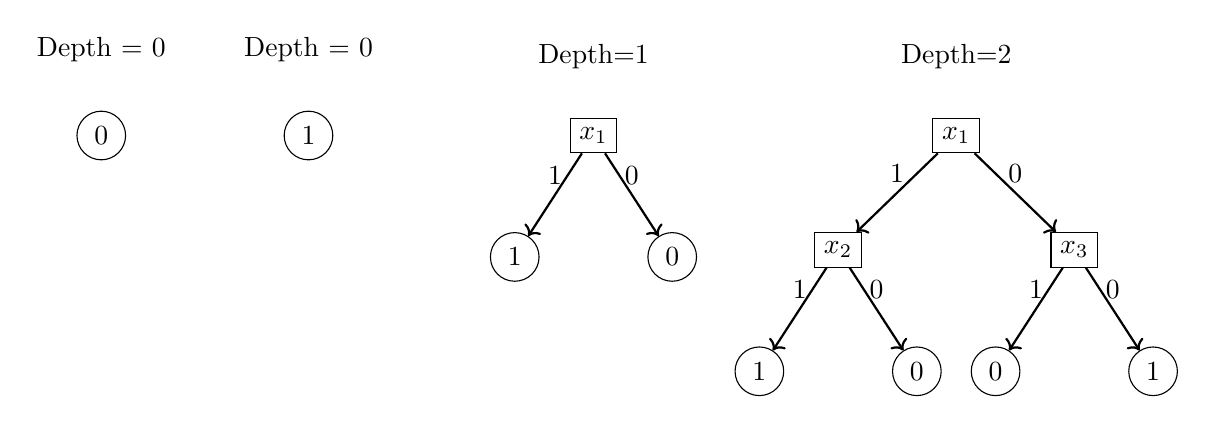
\begin{tikzpicture}
  \node[draw, circle] (false) at (0,0) {$0$};
  \node[above=0.5cm of false] {Depth = 0};

  \node[draw, circle, right=2cm of false] (true)  {$1$};
  \node[above=0.5cm of true] {Depth = 0};

  \node[draw, rectangle, right=3cm of true] (t21) {$x_1$};
  \node[draw, circle, below=1cm of t21, xshift=-1cm] (t22) {$1$};
  \node[draw, circle, below=1cm of t21, xshift=1cm] (t23) {$0$};
  \draw[->,thick] (t21) -- node[midway, above] {$1$} (t22);
  \draw[->,thick] (t21) -- node[midway, above] {$0$} (t23);  

  \node[above=0.5cm of t21] {Depth=1};

  \node[draw, rectangle, right=4cm of t21] (t31) {$x_1$};
  \node[draw, rectangle, below=1cm of t31, xshift=-1.5cm] (t32) {$x_2$};
  \node[draw, rectangle, below=1cm of t31, xshift=1.5cm] (t33) {$x_3$};
  \node[draw, circle, below=1cm of t32, xshift=-1cm] (t34) {$1$};
  \node[draw, circle, below=1cm of t32, xshift=1cm] (t35) {$0$};
  \node[draw, circle, below=1cm of t33, xshift=-1cm] (t36) {$0$};
  \node[draw, circle, below=1cm of t33, xshift=1cm] (t37) {$1$};

  \draw[->,thick] (t31) -- node[midway, above] {$1$} (t32);
  \draw[->,thick] (t31) -- node[midway, above] {$0$} (t33);

  \draw[->,thick] (t32) -- node[midway, above] {$1$} (t34);
  \draw[->,thick] (t32) -- node[midway, above] {$0$} (t35);
  \draw[->,thick] (t33) -- node[midway, above] {$1$} (t36);
  \draw[->,thick] (t33) -- node[midway, above] {$0$} (t37);    
  \node[above=0.5cm of t31] {Depth=2};  
\end{tikzpicture}

\begin{enumerate}
\item Since decision trees represent a finite hypothesis class, the quantity of
  interest is the number of such trees---i.e., trees with depth $k$ over $n$
  features. Suppose we use $S_n(k)$ to denote the number of the number of trees
  with depth exactly $k$ if we have $n$ features.

  The following questions guide you through this counting process. Recall that
  each answer should be accompanied with an explanation.\emph{If you simply
    write the final answer, you will not get any points.} (\textbf{Please see the note at the end of this questions for further clarification}3).

  \begin{enumerate}
  \item \relax[2 points] What is $S_n(0)$? That is how many trees of depth $0$
    exist?
    
  \item \relax[3 points] What is $S_n(1)$? That is, with $n$ features, how many
    trees of depth $1$ exist?
    
  \item \relax[4 points] Suppose you know the number of trees with depth $i$,
    for some $i$. This quantity would be $S_n(i)$ using our notation. Write down
    a recursive definition for $S_n(i+1)$ in terms of $n$ and $S_n(i)$.

    For this expression, you can assume that we are allowed to the use same
    feature any number of times when the tree is constructed.

  \item \relax[6 points] Recall that the quantity of interest for PAC bounds is
    the $\log$ of the size of the hypothesis class. Using your answer for the
    previous questions, find a closed form expression representing $\log S_n(k)$
    in terms of $n$ and $k$. Since we are not looking for an exact expression,
    but just an order of magnitude, so you can write your answer in the big $O$
    notation.
    
  \end{enumerate}

\item Next, you will use your final answer from the previous question to state a
  sample complexity bound for decision trees of depth $k$.

  \begin{enumerate}
  \item \relax[3 points] With finite hypothesis classes, we saw two Occam's
    razor results. The first one was for the case of a consistent learner and
    the second one was for the agnostic setting. For the situation where we are
    given a dataset and asked to use depth-$k$ decision trees as our hypothesis
    class, which of these two settings is more appropriate? Why?

  \item \relax[4 points] Using your answers from questions so far, write the
    sample complexity bound for the number of examples $m$ needed to guarantee
    that with probability more than $1- \delta$, we will find a depth-$k$
    decision tree whose generalization error is no more than $\epsilon$ away
    from its training error.

  \end{enumerate}

\item \relax[4 points] Is the set of depth-$k$ decision trees PAC learnable? Is
  it efficiently PAC learnable?

\item \relax[4 points] Suppose the number of features we have is large and the
  depth limit we are considering is also large (say, in the thousands or
  more). Will the number of examples we need be small or large? Discuss the
  implications of the sample complexity bound from above.
  
\end{enumerate}

\textbf{NOTE}: In this question we are counting trees that are structurally different instead of functionally different. As an exercise, you can confirm that the following two trees are structurally different but equal in terms of the label they assign to any example, namely the trees are functionally equivalent.


\begin{center}
    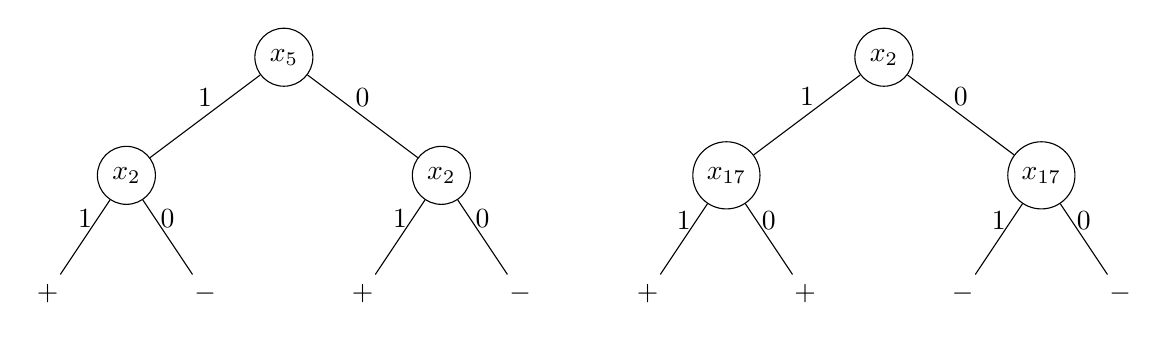
\begin{tikzpicture}[grow = down, level/.style={sibling distance=40mm/#1}, node/.style = {draw, circle}]
    \begin{scope}
      \node[node] {$x_5$} % root
      child { node[node] {$x_2$}
      child { node {$+$}
          edge from parent node [above] {1}}
      child { node {$-$}
          edge from parent node [above] {0}}
        edge from parent node [above] {1}}
      child { node[node] {$x_2$} % x_2
        child { node {$+$}
          edge from parent node [above] {1}}
        child { node {$-$}
          edge from parent node [above] {0}}
        edge from parent node [above] {0}};
    \end{scope}
    \begin{scope}[xshift=3in]
     \node[node] {$x_2$} % root
      child { node[node] {$x_{17}$}
      child { node {$+$}
          edge from parent node [above] {1}}
      child { node {$+$}
          edge from parent node [above] {0}}
        edge from parent node [above] {1}}
      child { node[node] {$x_{17}$} % x_2
        child { node {$-$}
          edge from parent node [above] {1}}
        child { node {$-$}
          edge from parent node [above] {0}}
        edge from parent node [above] {0}};
    \end{scope}
    \end{tikzpicture}
  \end{center}




\section{Shattering [15 points, for 6350 students]}
\label{sec:shattering}

Suppose we have a set $X_n$ consists of all binary sequences of a length $n$.
For example, if $n=3$, the set would consist of the eight elements
\texttt{\{000, 001, 010, 011, 100, 101, 110, 111\}}.

Consider a set of functions $H_n$ that we will call the set of {\em
  templates}. Each template is a sequence of length $n$ that is constructed
using {\tt 0}, {\tt 1} or {\tt -} and returns $+1$ for input binary sequences
that match it and $-1$ otherwise. While checking whether a template matches an
input, a {\tt -} can match both a {\tt 0} and a {\tt 1}.

For example, the template {\tt -10} matches the binary strings {\tt 010} and
{\tt 110}, while {\tt -1-} matches all strings that have a {\tt 1} in the middle
position, namely {\tt 010}, {\tt 011}, {\tt 110} and {\tt 111}.

Does the set of templates $H_n$ shatter the set $X_n$? Prove your answer.


\section{VC Dimension [45 points]}
\label{sec:vc-dimension}
\begin{enumerate}
\item ~[5 points] Assume that the three points below can be labeled in any way.  Show with pictures how they can be shattered by a linear classifier.  Use filled dots to represent positive classes and unfilled dots to represent negative classes.

  \begin{tikzpicture}
    \begin{axis}[my style, xtick={-1,0,...,3}, ytick={-1,0,...,3},
      xmin=-1, xmax=3, ymin=-1, ymax=3]
      \addplot[mark=*,only marks] coordinates {(2,2)(1,1)(1,2)};
    \end{axis}
  \end{tikzpicture}
  
\item {\bf VC-dimension of axis aligned rectangles in $\mathbb{R}^d$}:
  Let $H^d_{rec}$ be the class of axis-aligned rectangles in
  $\mathbb{R}^d$. When $d=2$, this class simply consists of rectangles
  on the plane, and labels all points strictly outside the rectangle
  as negative and all points on or inside the rectangle as positive.
  In higher dimensions, this generalizes to $d$-dimensional boxes,
  with points outside the box labeled negative.

  \begin{enumerate}
  \item ~[10 points] Show that the VC dimension of $H^2_{rec}$ is 4.
  \item ~[10 points] Generalize your argument from the previous proof
    to show that for $d$ dimensions, the VC dimension of $H^d_{rec}$
    is $2d$.
  \end{enumerate}
  
\item In the lectures, we considered the VC dimensions of infinite
  concept classes. However, the same argument can be applied to finite
  concept classes too. In this question, we will explore this setting.

  \begin{enumerate}
  \item ~[10 points] Show that for a finite hypothesis class
    $\mathcal{C}$, its VC dimension can be at most
    $\log_2\left(|\mathcal{C}|\right)$. (Hint: You can use
    contradiction for this proof. But not necessarily!)

  \item ~[5 points] Find an example of a class $\mathcal{C}$ of
    functions over the real interval $X = [0,1]$ such that
    $\mathcal{C}$ is an {\bf infinite} set, while its VC dimension is
    exactly one.

  \item ~[5 points] Give an example of a {\bf finite} class
    $\mathcal{C}$ of functions over the same domain $X = [0,1]$ whose
    VC dimension is exactly $\log_2(|\mathcal{C}|)$.

  \end{enumerate}
  
\end{enumerate}


\section{Extra Credit - Decision Lists [25 points]}
In this problem, we are going to learn the class of $k$-decision
lists. A decision list is an ordered sequence of if-then-else
statements. The sequence of if-then-else conditions are tested in
order, and the answer associated to the first satisfied condition is
output. See Figure~\ref{fig:decision_list} for an example of a
$2$-decision list.

\begin{figure}[h]
\begin{center}
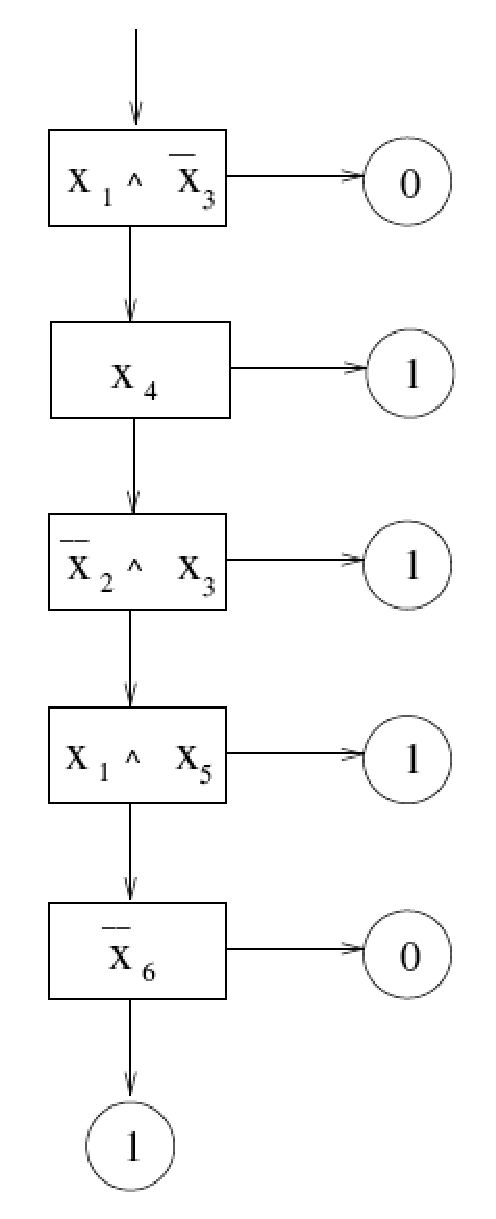
\includegraphics[width=1.35in]{fig-1.pdf}
\caption{A $2$-decision list.}
\label{fig:decision_list}
\end{center}
\end{figure}

A {\em $k$-decision list} over the variables $x_{1}, \ldots, x_{n}$ is
an ordered sequence $L=(c_{1}, b_{1}), \ldots, (c_{l},b_{l})$ and a
bit $b$, in which each $c_{i}$ is a conjunction of at most $k$
literals over $x_{1},\ldots, x_{n}$. The bit $b$ is called the {\em
  default} value, and $b_{i}$ is referred to as the bit {\em
  associated} with condition $c_{i}$. For any input $x \in \{0,
1\}^{n}$, $L(x)$ is defined to be the bit $b_{j}$, where $j$ is the
smallest index satisfying $c_{j}(x)=1$; if no such index exists, then
$L(x)=b$.

We denote by $k\mbox{\em -DL}$ the class of concepts that can be
represented by a $k$-decision list.


\begin{enumerate}
\item \relax[8 points] Show that if a concept $c$ can be represented
  as a $k$-decision list so can its complement, $\neg c$. You can show
  this by providing a $k$-decision list that represents $\neg c$,
  given $c = \{(c_{1},b_{1}), \ldots, (c_{l},b_{l}),b)$.

\item \relax[9 points] Use  Occam's Razor to show: \\
  For any constant $k \geq 1$, the class of $k$-decision lists is
  PAC-learnable.

\item \relax[8 points] Show that $1$-decision lists are a linearly
  separable functions. (Hint: Find a weight vector that will make the
  same predictions a given $1$-decision list.)

\end{enumerate}





\end{document}

%%% Local Variables:
%%% mode: latex
%%% TeX-master: t
%%% End:
